\documentclass{article}

\usepackage[a4paper, total={6.5in, 11in}]{geometry}
\setlength{\parindent}{0em}

\usepackage{latex/common}

\usepackage{graphicx}
\graphicspath{{titech/ART.T458.AdvancedMachineLearning/Final1/}}

\newcommand{\under}[2]{\mathop{#1}\limits_{#2}}
\newcommand{\s}{\sum\limits_{i=1}^{n}}
\newcommand{\p}[2]{\frac{\partial #1}{\partial #2}}
\newcommand{\pp}[3]{\frac{{\partial}^2 #1}{\partial #2 \partial #3}}
\newcommand{\B}[1]{\left\{\begin{aligned}#1\end{aligned}\right.}
\newcommand{\E}{\mathrm{E}}
\newcommand{\V}{\mathrm{V}}

\title{Final Report}
\date{2021\\ July}
\author{Sixue Wang, Tokyo Institute of Technology}

\begin{document}

\maketitle

\section*{Problem 1}

\newcommand{\e}{exp(-y_i w^T x_i)}
\newcommand{\ee}{exp(-2y_i w^T x_i)}

The loss function is $ J(w) = \s ln(1+exp(-y_i w^T x_i)) + \lambda w^Tw $ \\
Assume that $P(y_i|w,x_i) = \frac{1}{1+exp(-y_iw^Tx_i)}$

\subsection*{1.1 Batch Steepest Gradient Descent}

The steepest gradient method using the opposite gradient of loss function with respect to weights as the direction of descent. That means the weights minus the gradient scaling by the learning rate in every iteration. The batch mode means, we only use part of the data to update the weights.\\

So the first step is deriving the gradient: \\

\begin{CMath}
  gradient = \p{J(w)}{w}           &= \s \frac{\e}{1+\e} (-y_ix_i) + 2\lambda w \\
                                   &= \s (1-P(y_i|w,x_i))(-y_ix_i) + 2\lambda w
\end{CMath}

\begin{PYCode}[Batch SGD]
  D <- Data, W <- 0, B <- batch size, lr <- leanring rate
  for i in range(epoch):
    d <- D random shuffle
    for xi, yi in zip(split(D, B)): # split data into batch by batch size
      W += -lr * gradient(xi, yi)
\end{PYCode}

\subsection*{1.2 Newton Method}

Newton method is a second-order method. The main idea is precondition the gradient by the inverse Hessian matrix of the loss function with respect to weights.\\

Now let's derive the Hessian: \\

\begin{CMath}
H = \pp{J(w)}{w}{w^T} &= \p{}{w^T} \s (1-P(y_i|w,x_i))(-y_ix_i) + 2\lambda w \\
                      &= \s \p{}{w^T}(P(y_i|w,x_i)(-y_ix_i)) + 2\lambda I \\
                      &= \s P(y_i|w,x_i)(1-P(y_i|w,x_i)) (-y_ix_i)\p{}{w}(-y_iw^Tx_i) + 2\lambda I \\
                      &= \s P(y_i|w,x_i)(1-P(y_i|w,x_i)) (-y_ix_i)(-y_ix_i^T) + 2\lambda I \\
                      &= \s P(y_i|w,x_i)(1-P(y_i|w,x_i)) x_ix_i^T + 2\lambda I
\end{CMath}

\begin{PYCode}[Newton Method]
  X <- Feature, Y <- Label, W <- 0, lr <= learning rate
  for i in range(epoch):
    W += -lr * inverse(H(X, Y)) * gradient(X, Y)
\end{PYCode}

\subsection*{1.3 Comparison between SGD and Newton Method}

\begin{center}
  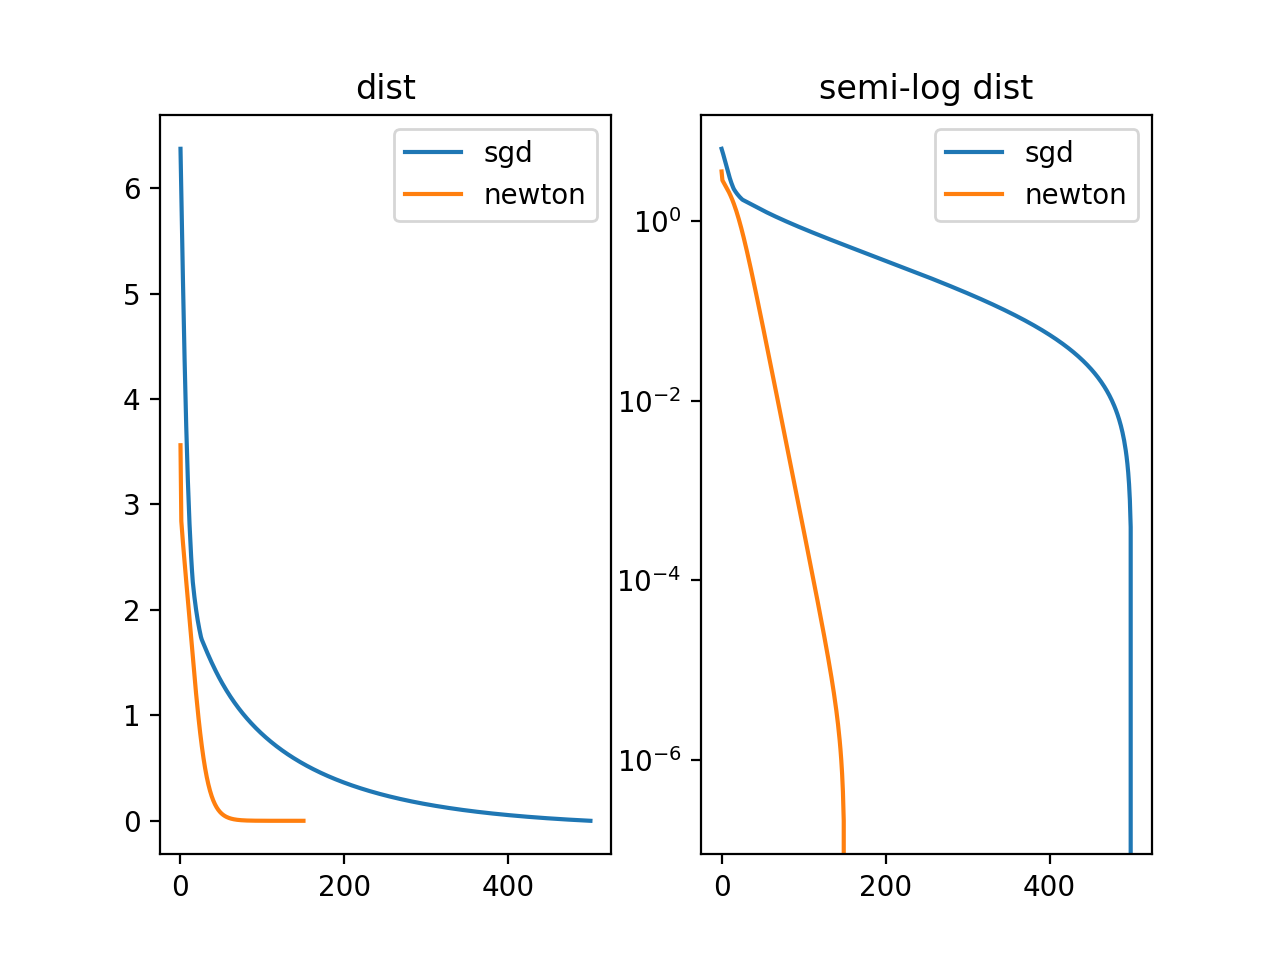
\includegraphics[scale=0.7]{semi-log}
\end{center}

\subsection*{1.4 Multiclass}

Before solving multiclass problem, I need to introduce softmax:
\begin{CMath}
  softmax(x)[i] = \frac{e^x[i]}{sum(e^x)}
\end{CMath}
It process vector in element-wise mode.\\

Now we can use cross-entropy loss with l2-norm to optimize multiclass version of logistic regression:
\begin{CMath}
  L(w) = -log(softmax(w^Tx)[y])) + 2 \lambda w
\end{CMath}
where $x \in R^d$, $w \in R^{dxC}$, $y \in [1, C]$ indicates the class, and $C$ is the number of the classes, . There is only one thing left to implement SGD and Newton Method, which is deriving the gradient and the Hessian.
\begin{CMath}
  gradient &= softmax(w^Tx) - one\_hot(y) + 2\lambda w \\
  H        &= Diag(softmax(w^Tx)) - softmax(w^Tx)softmax(w^Tx)^T + 2\lambda \\
\end{CMath}
where Diag expands the vector to a diagonal matrix.

\begin{center}
  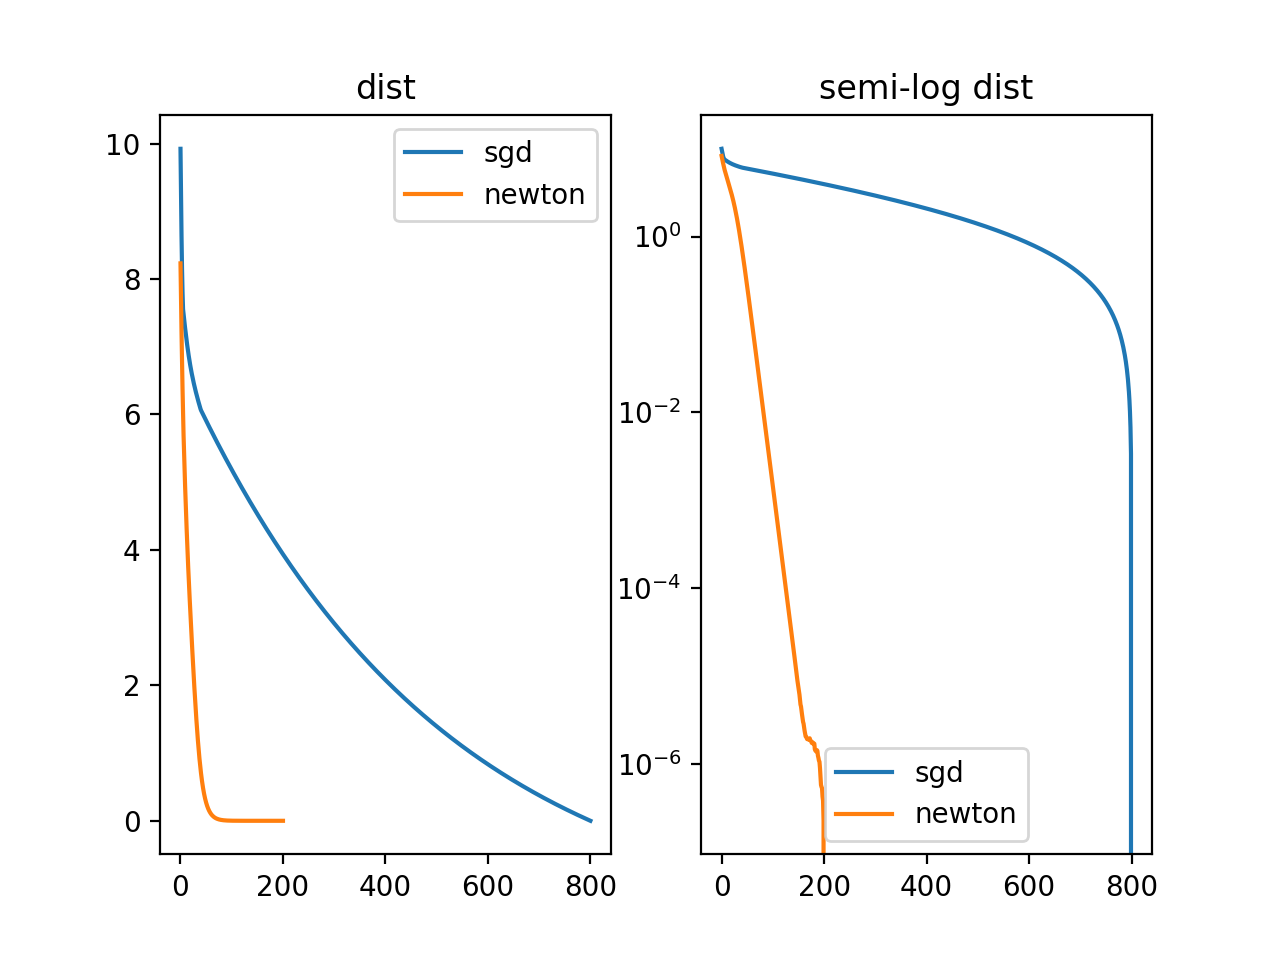
\includegraphics[scale=0.7]{semi-log2}
\end{center}

\newpage


\section*{Problem 2}
The problem is
\begin{CMath}
  \hat{w} = \mathop{argmin}_{w} ((w-\mu)^T A (w-\mu) + \lambda ||w||_1)
\end{CMath}
The updating rule is
\begin{CMath}
  w^{t+1} = ST_{\eta\lambda}(w^t - 2 \eta A (w-\mu))
\end{CMath}

\begin{center}
  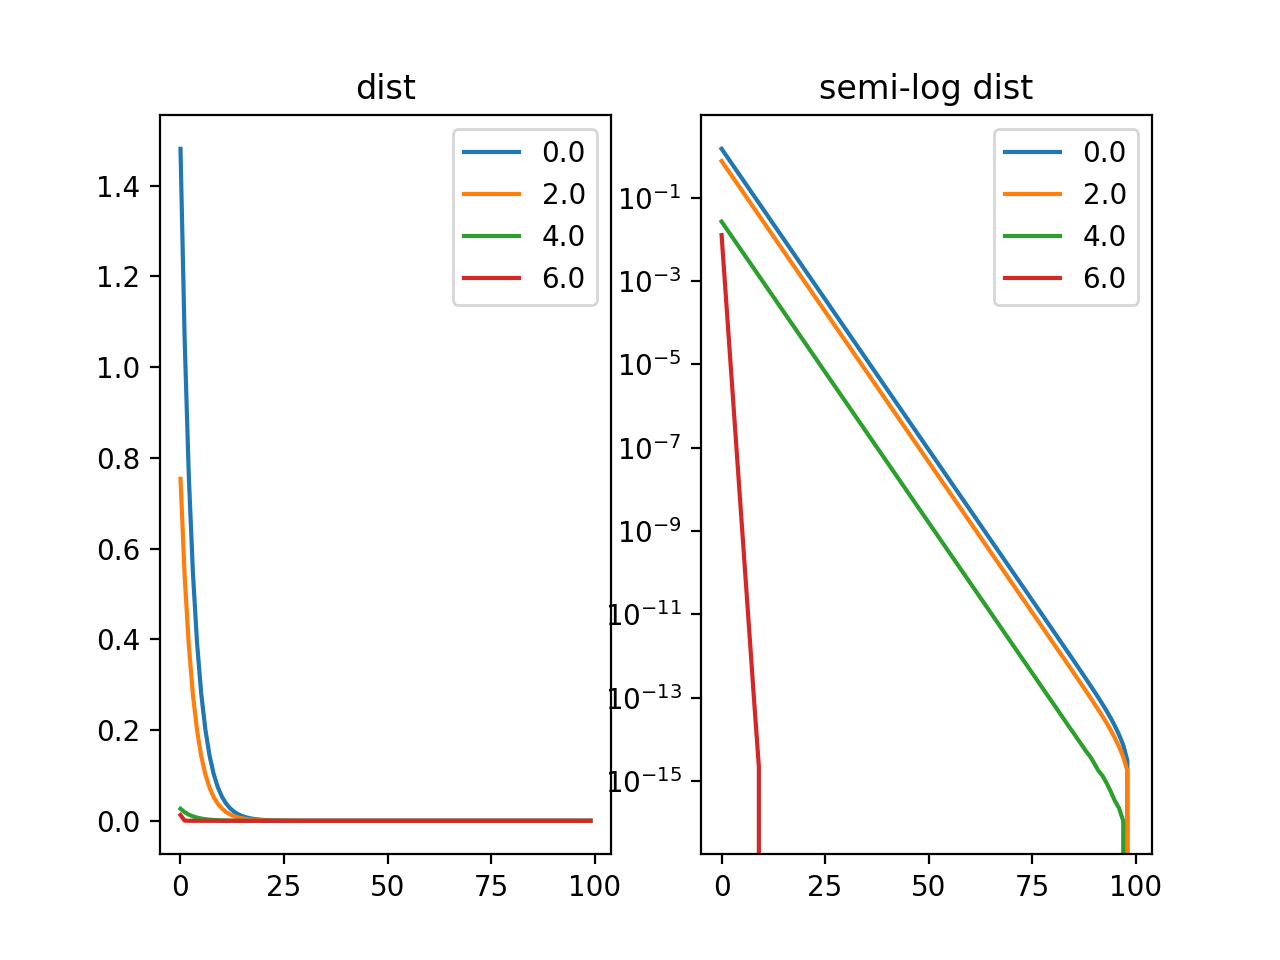
\includegraphics[scale=0.7]{lasso.png}
\end{center}


\section*{Problem 3}
\subsection*{3.1}
Let rewrite the problem in convex problem form:
\begin{CMath}
  minimize_{w,\xi} \quad & \frac{1}{2}w^Tw + \frac{1}{2\lambda}1^T\xi \\
  subject \; to    \quad & \xi_i \geq 1-y_iw^Tx_i, \quad i=1,...,n \\
                         & \xi \geq 0 \\
\end{CMath}
The Lagrangian of the original problem is:
\begin{CMath}
  L(w, \xi, \alpha, \beta) = \frac{1}{2}w^Tw + \frac{1}{2\lambda}1^T\xi + \s \alpha_i (1-y_i w^T x_i-\xi_i) - \beta^T\xi \\
\end{CMath}
Now we can get the optimal value at the critial point of the Lagrangian function.
\begin{CMath}
  & \p{L}{w}|_{w=\hat{w}} & = w - \s \alpha_i y_i x_i = 0 & \implies \hat{w} = \s \alpha_i y_i x_i \\
  & \p{L}{\xi}|_{\xi=\hat{\xi}} & = \frac{1}{2\lambda}1 - \alpha - \beta = 0 & \implies \alpha + \beta = \frac{1}{2\lambda}1 \\
\end{CMath}
After substituing the previous result back into the Lagrangian, we can get the dual function:
\begin{CMath}
  \tilde{L}(\alpha, \beta) &= \frac{1}{2} w^T \s \alpha_i y_i x_i + \frac{1}{2\lambda}1^T\xi + \s \alpha_i - \s \alpha_i y_i w^T x_i - \s \alpha_i \xi_i - \beta^T\xi \\
                           &= \frac{1}{2} w^T \s \alpha_i y_i x_i - w^T \s \alpha_i y_i x_i + \alpha^T1 + \frac{1}{2\lambda}1^T\xi - \alpha^T\xi - \beta^T\xi \\
                           &= -\frac{1}{2} w^T \s \alpha_i y_i x_i + \alpha^T1 + (\frac{1}{2\lambda}1 - \alpha - \beta)^T\xi \\
                           &= -\frac{1}{2} \s \alpha_i y_i x_i^T \s \alpha_i y_i x_i + \alpha^T1 + 0^T\xi \\
                           &= -\frac{1}{2} \alpha^T K \alpha + \alpha^T1 \\
  \tilde{L}(\alpha)        &= -\frac{1}{2} \alpha^T K \alpha + \alpha^T1 \\
\end{CMath}
On the other hand, from $\alpha + \beta = \frac{1}{2\lambda}1$ and $\alpha \geq 0$, $\beta \geq 0$, we have $0 \leq \alpha \leq \frac{1}{2\lambda}1$
\begin{CMath}
  maximize_{\alpha} \quad & -\frac{1}{2} \alpha^T K \alpha + \alpha^T1 \\
  subject \; to     \quad & 0 \leq \alpha \leq \frac{1}{2\lambda}1 \\
\end{CMath}
To get the exactly same result in the question, only one thing need to do is rescaling $\alpha$:
\begin{CMath}
  maximize_{\alpha} \quad & -\frac{1}{2} \frac{1}{2\lambda}\alpha^T K \frac{1}{2\lambda}\alpha + \frac{1}{2\lambda}\alpha^T1 \\
  subject \; to     \quad & 0 \leq \alpha \leq 1 \\
  maximize_{\alpha} \quad & -\frac{1}{4\lambda} \alpha^T K \alpha + \alpha^T1 \\
  subject \; to     \quad & 0 \leq \alpha \leq 1 \\
\end{CMath}


\section*{Problem 8}
\subsection*{8.1}
To get the optimal $\hat{w}_{LS}$ and $\hat{w}_{ridge}$, we need to get the critial point with respect to $w$. \\

\begin{CMath}
  \p{}{w} \frac{1}{2} ||y-Xw||^2_2 \mid _{w=\hat{w}_{LS}} &= 0 \\
  \frac{1}{2} 2 (-X^T) (y-X\hat{w}_{LS})         &= 0 \\
  -X^Ty + X^TX\hat{w}_{LS} &= 0 \\
  (X^TX)\hat{w}_{LS} &= X^Ty \\
  \hat{w}_{LS} &= (X^TX)^{-1}X^Ty \\
  \p{}{w} \frac{1}{2} ||y-Xw||^2_2 + \lambda ||w||^2_2 \mid _{w=\hat{w}_{ridge}} &= 0 \\
  \frac{1}{2} 2 (-X^T) (y-X\hat{w}_{ridge}) + \lambda 2 \hat{w}_{ridge}                  &= 0 \\
  -X^Ty + X^TX\hat{w}_{ridge} + \lambda \hat{w}_{ridge} &= 0 \\
  (X^TX + \lambda I)\hat{w}_{ridge} &= X^Ty \\
  \hat{w}_{ridge} &= (X^TX + \lambda I)^{-1}X^Ty
\end{CMath}

\subsection*{8.2}
$X^TX$ is a symmetric matrix, so there exists an invertible matrix $P$ and a non-negative diagonal matrix $D$ such that $X^TX = PDP^{-1}$, and all the elements of $D$ are the eigenvalue of the $X^TX$. On the other hand $(X^TX+\lambda I) = P(D+\lambda I)P^{-1}$, so all eigenvalues of $X^TX+\lambda I$ are greater than zero, so it is regular.


\subsection*{8.3}
\begin{CMath}
  ||X\hat{w}_{LS}||^2_2 &= y^TXPD^{-1}P^{-1}X^Ty \\
  ||X\hat{w}_{ridge}||^2_2 &= y^TXP(D+\lambda I)^{-1}D(D+\lambda I)^{-1}P^{-1}X^Ty
\end{CMath}

Let's focus on the comparison between $D^{-1}$ and $(D+\lambda I)^{-1}D(D+\lambda I)^{-1}$. Benefit from the diagonal matrix, we can consider only one element at a time.

\begin{CMath}
  d_i &< d_i + \lambda \\
  d_i(d_i + \lambda)^{-1} &< 1 \\
  d_i^{-1} &> (d_i + \lambda)^{-1} > (d_i + \lambda)^{-1}d_i(d_i + \lambda)^{-1}
\end{CMath}

so $||X\hat{w}_{LS}||^2_2 > ||X\hat{w}_{ridge}||^2_2$

\section*{Problem 9}
\subsection*{9.1}
Minimuming the Euclidean distance is equivalent to minimuming the squared Euclidean distance, so:

\begin{CMath}
  (x_i-x)^2+(y_i-x)^2 \\
  x_i^2 - 2 x x_i + x^2 + y_i^2 - 2 y_i y + y^2 \\
  (x^2 + y^2) + (x_i^2 - 2 x x_i + y_i^2 - 2 y_i y)
\end{CMath}

For a specific $point(x ,y)$, the maximum distance is fixed and assume that point is $(x_{max}, y_{max})$, then:
\begin{CMath}
  (x^2 + y^2) + (x_{max}^2 - 2 x x_{max} + y_{max}^2 - 2 y_{max} y) \\
  \lambda = (x_{max}^2 - 2 x x_{max} + y_{max}^2 - 2 y_{max} y)
\end{CMath}
and the distance of other points must be less or equal than $\lambda$, rewrite this idea in quadratic programming problem:
\begin{CMath}
  minimize_{\lambda \in R, x \in R, y \in R}\; & x^2+y^2+\lambda \\
  subject \; to \; & x_i^2 - 2 x x_i + y_i^2 - 2 y_i y <= \lambda
\end{CMath}

\section*{Feedback}

Thank you for your excellent lecture. I also want to learn second-order optimization methods, such as Hessian-free methods, K-FAC, and so on. Another topic is HMM, I think this method is widely used in speech.

\end{document}
